\chapter{तंत्रिकीय सुघट्यता, अधिगम और स्मृति}\label{ch:b3:learning-memory}

1953 में किसी शल्यचिकित्सक ने असाध्य अपस्मार से पीड़ित किसी युवक के
दोनों शंख-खंडों का भीतरी हिस्सा निकाल दिया। दौरे थम गए; और वह रोगी,
जिसे पचास वर्षों तक H.M. के नाम से जाना गया, किसी घटना की कोई और टिकाऊ
स्मृति फिर कभी नहीं बना सका। वह बातचीत कर सकता था, किसी आईने में तारा
बनाना किसी भी और की तरह सीख सकता था --- और हर दिन यह नकार सकता था कि
उसने वह काम कभी देखा भी हो --- और उसे अपना बचपन याद था। पता चला कि
स्मृति एक चीज़ नहीं है, और घटनाओं की नई स्मृतियाँ बनाना अँगूठे जितनी
किसी संरचना पर टिका है। सीखते समय किसी मस्तिष्क में क्या बदलता है, यह
तंत्रिका-विज्ञान का सबसे पुराना प्रश्न है, और उसका उत्तर, जो बीस हज़ार
न्यूरॉनों वाली किसी समुद्री स्लग में और चूहे के \omterm{def:b3:learning-memory:kinds}{हिप्पोकैम्पस} की काटों
में निकाला गया, यह है कि तंत्रिका-संधियाँ अपना बल उसके हिसाब से बदल
लेती हैं जो उनसे होकर गुज़रता है --- यानी वही नियम जो डोनल्ड हेब ने
1949 में अटकल से निकाला और जिसे लागू करना किसी अणु, यानी \omterm{prop:b3:learning-memory:nmda}{NMDA ग्राही},
के ज़िम्मे निकला। यह अध्याय उसी नियम और उसके तंत्र की बात करता है, उन
परिपथों की जो उसे स्थान और घटनाएँ संचित करने में काम में लेते हैं, उस
गणित की जो बताता है कि ऐसा कोई तंत्र क्या सीख सकता है और कितना रख सकता
है, और उस पुरस्कार-संकेत की जो उसे बताता है कि सीखने लायक क्या है।

\section{स्मृति के प्रकार और उनका ठिकाना}

\begin{definition}[अधिगम और स्मृति के रूप]\label{def:b3:learning-memory:kinds}
\index{अभ्यस्तीकरण}\index{संवेदीकरण}\index{अनुबंधन}\index{घोषणात्मक स्मृति}\index{प्रक्रियात्मक स्मृति}\index{सुदृढ़ीकरण}\index{हिप्पोकैम्पस}
सबसे सरल अधिगम \emph{असाहचर्यी} है: \emph{अभ्यस्तीकरण}, यानी किसी
बार-बार दुहराए गए हानिरहित उद्दीपक पर घटती अनुक्रिया, और
\emph{संवेदीकरण}, यानी किसी हानिकारक उद्दीपक के बाद बढ़ी हुई अनुक्रिया।
\emph{साहचर्यी} अधिगम दो घटनाएँ जोड़ता है: \emph{चिरप्रतिष्ठित
अनुबंधन} (पावलोव) में कोई उदासीन उद्दीपक, जो किसी पुरस्कार या दंड का
पूर्वानुमान करे, स्वयं वह अनुक्रिया खींचने लगता है;
\emph{क्रियाप्रसूत अनुबंधन} में जिस क्रिया को पुरस्कार मिले वह
दुहराई जाती है। मानव स्मृति \emph{घोषणात्मक} स्मृति में बँटती है ---
तथ्य और घटनाएँ, जो सचेत रूप से याद आते हैं और \emph{हिप्पोकैम्पस} तथा
मध्यवर्ती शंख-खंड पर टिके हैं --- और \emph{अघोषणात्मक} स्मृति में ---
कौशल तथा आदतें (धारीदार पिंड, \omterm{def:b3:nervous-systems:plan}{अनुमस्तिष्क}), अनुबंधित भय (अमिग्डला),
पूर्वप्रभावन (प्रांतस्था) --- जो बिना याद आए निष्पादन में प्रकट होती
है। कोई स्मृति पहले किसी अस्थिर अल्पकालिक रूप में रहती है, जो सेकंडों
से घंटों तक चलता है, और घंटों से वर्षों में किसी ऐसे स्थिर दीर्घकालिक
रूप में \emph{सुदृढ़} हो जाती है जिसे हिप्पोकैम्पस की ज़रूरत नहीं रहती
और जो प्रांतस्था में बसता है।
\end{definition}

\begin{proof}[प्रमाण-सामग्री]
स्कोविल और मिलनर (1957) ने H.M. की सूचना दी: दोनों \omterm{def:b3:learning-memory:kinds}{हिप्पोकैम्पस} और
पड़ोसी प्रांतस्था हटाए जाने के बाद उसकी बुद्धि और शल्यक्रिया से पहले की
उसकी स्मृतियाँ बड़े हिस्से में अक्षत थीं, उसकी कार्यकारी स्मृति तब तक
सामान्य थी जब तक वह किसी चीज़ पर ध्यान दिए रहे, पर वह किसी भी घटना या
तथ्य की कोई नई स्मृति नहीं बना सका। उसने प्रेरक कौशल दिनों भर में
सामान्य दर से सीखे, यह नकारते हुए कि उसने कभी अभ्यास किया --- इसलिए
कौशल-स्मृति को \omterm{def:b3:learning-memory:kinds}{हिप्पोकैम्पस} नहीं चाहिए --- और उसे दूर का अतीत
शल्यक्रिया से ठीक पहले के वर्षों से बेहतर याद था, इसलिए \omterm{def:b3:learning-memory:kinds}{हिप्पोकैम्पस}
\omterm{def:b3:learning-memory:kinds}{घोषणात्मक स्मृतियाँ} बिछाने और कुछ समय तक थामे रहने के लिए चाहिए था,
उन्हें सदा के लिए संचित करने के लिए नहीं। मिलती-जुलती क्षतियों वाले
बंदरों और चूहों ने वही विलगाव दिखाया, और किसी एक रोगी के अध्ययन ने उस
क्षेत्र को नए सिरे से खड़ा कर दिया।
\end{proof}

\section{हेब का नियम और उसका अणु}

\begin{definition}[हेबीय सुघट्यता, LTP और LTD]\label{def:b3:learning-memory:ltp}
\index{हेब का नियम}\index{दीर्घकालिक प्रबलन}\index{दीर्घकालिक अवसादन}\index{आवेग-काल-निर्भर सुघट्यता}
हेब (1949) ने प्रस्ताव किया कि जब कोई पूर्वसंधिक न्यूरॉन बार-बार किसी
पश्चसंधिक न्यूरॉन को दगाने में हिस्सा ले, तब उनके बीच का जोड़ मज़बूत
होता है --- ``जो कोशिकाएँ साथ दगती हैं वे साथ जुड़ जाती हैं''।
\emph{दीर्घकालिक प्रबलन} (LTP) उसका प्रायोगिक रूप है: किसी पथ के
उच्च-बारंबारता उद्दीपन का कोई छोटा झोंका उन तंत्रिका-संधियों को, जो
उसने सक्रिय कीं, किसी काट में घंटों तक और किसी प्राणी में हफ़्तों तक
मज़बूत छोड़ जाता है। LTP \emph{निवेश-विशिष्ट} है (केवल उद्दीपित संधियाँ
बदलती हैं), \emph{साहचर्यी} है (उसी कोशिका पर किसी प्रबल निवेश के साथ
जोड़ा गया कोई दुर्बल निवेश प्रबलित होता है) और उसे कोशिका विध्रुवित
करने के लिए निवेशों में \emph{\omterm{def:b3:structural-biology:allostery}{सहकारिता}} चाहिए। \emph{दीर्घकालिक
अवसादन} (LTD) उसका उलटा है, जो लंबी चली निम्न-बारंबारता क्रियाशीलता से
बनता है। \emph{आवेग-काल-निर्भर सुघट्यता} में चिह्न क्रम से तय होता है:
पश्चसंधिक आवेग से कुछ मिलीसेकंड \emph{पहले} पड़ा कोई पूर्वसंधिक आवेग उस
संधि को मज़बूत करता है, और ठीक \emph{बाद} पड़ा कोई उसे कमज़ोर, और यह
दोनों ओर लगभग \qty{20}{ms} की किसी खिड़की के भीतर --- ताकि कोई संधि
केवल सहसंबंध नहीं, पूर्वानुमान करना सीखे।
\end{definition}

\begin{proposition}[संपात-संसूचक के रूप में NMDA ग्राही]\label{prop:b3:learning-memory:nmda}
\index{NMDA ग्राही}\index{AMPA ग्राही}\index{CaMKII}\index{CREB}\index{द्रुमिका कंटक}
उत्तेजी तंत्रिका-संधियों पर ग्लूटामेट दो ग्राहियों पर काम करता है।
\emph{AMPA} ग्राही बँधते ही खुल जाता है और साधारण संधि-धारा ढोता है।
\emph{NMDA} ग्राही ग्लूटामेट बाँधता है पर विश्राम विभव पर उसके छिद्र
में बैठा कोई मैग्नीशियम आयन उसे रोके रखता है; केवल तब, जब पश्चसंधिक
झिल्ली विध्रुवित हो --- एक साथ आते अनेक निवेशों से, या किसी पीछे लौटते
क्रिया विभव से --- वह मैग्नीशियम बाहर निकलता है और वह वाहिका चालन करती
है, जिससे कैल्सियम भीतर आता है। इस तरह \omterm{prop:b3:learning-memory:nmda}{NMDA ग्राही} केवल तब खुलता है जब
पूर्वसंधिक मोचन (ग्लूटामेट) पश्चसंधिक क्रियाशीलता (विध्रुवण) के साथ
संपात करे: वह किसी एक ही प्रोटीन में हेब का ``और'' द्वार है। किसी
\emph{\omterm{prop:b3:learning-memory:nmda}{द्रुमिका कंटक}} में घुसा वह कैल्सियम काइनेज़ \emph{CaMKII} सक्रिय
करता है, जो \omterm{prop:b3:learning-memory:nmda}{AMPA ग्राहियों} का फ़ॉस्फ़ोरिलन करती है और किसी भंडार से और
भी ग्राही उस संधि में ठेल देती है --- वह संधि मिनटों में मज़बूत हो जाती
है (आरंभिक LTP)। कैल्सियम की कोई बड़ी, धीमी बढ़त इसके बजाय
फ़ॉस्फ़ेटेज़ कैल्सिन्यूरिन सक्रिय करती है, जो \omterm{prop:b3:learning-memory:nmda}{AMPA ग्राही} हटा देती है:
यानी LTD। कुछ घंटों से अधिक चलते प्रबलन (देर वाला LTP) को नया प्रोटीन
चाहिए: काइनेज़ केंद्रक तक पहुँचती हैं, अनुलेखन कारक \emph{CREB} जीन
चालू कर देता है, और वह कंटक बढ़ता है तथा बँट भी सकता है --- यानी
जीन-अभिव्यक्ति की वही ज़रूरत, जो अध्ययन किए गए हर प्राणी में
अल्पकालिक को दीर्घकालिक स्मृति से अलग करती है।
\end{proposition}

\begin{proof}[प्रमाण-सामग्री]
ब्लिस और लोमो (1973) ने खरगोश के \omterm{def:b3:learning-memory:kinds}{हिप्पोकैम्पस} में जाते वेधी पथ को
स्पंदों की किसी रेल से उद्दीपित किया और पाया कि उभारी गई अनुक्रिया उसके
बाद घंटों तक बड़ी रही --- यानी पहला LTP। कॉलिंग्रिज (1983) ने दिखाया कि
\omterm{prop:b3:learning-memory:nmda}{NMDA ग्राही} का कोई अवरोधक (AP5) LTP का प्रेरण रोक देता है पर साधारण
संधि-अनुक्रिया नहीं; मॉरिस (1986) ने चूहों के \omterm{def:b3:learning-memory:kinds}{हिप्पोकैम्पस} में AP5
चढ़ाया और पाया कि वे सामान्य रूप से तैरते तथा देखते हुए भी पानी के किसी
कुंड में छिपे मंच की जगह अब नहीं सीख पाते; और जिन चूहों में \omterm{prop:b3:learning-memory:nmda}{NMDA ग्राही}
केवल \omterm{def:b3:learning-memory:kinds}{हिप्पोकैम्पस} के \omterm{def:b3:learning-memory:hippocampus}{CA1} क्षेत्र में विलोपित था उनमें वहाँ न LTP था न
स्थानिक स्मृति। वही ग्राही, उसी जगह, उस संधि-परिवर्तन के लिए और उस
अधिगम के लिए आवश्यक था।
\end{proof}

\begin{omfigure}
\begin{tikzpicture}[every node/.style={font=\scriptsize}, >=stealth]
  % presynaptic terminal
  \draw[thick, omDef, fill=omDef!12] (0,2.2) .. controls (0,3.4) and (4,3.4) .. (4,2.2) -- (4,1.7) -- (0,1.7) -- cycle;
  \node at (2,2.8) {पूर्वसंधिक सिरा};
  \foreach \p in {(0.8,2.0),(1.6,2.1),(2.6,2.0),(3.3,2.1)} \draw[thick, fill=omDef!40] \p circle (0.17);
  \foreach \p in {(1.2,1.45),(2.0,1.5),(2.9,1.42)} \fill[omProp] \p circle (0.06);
  \node[right, omProp] at (3.3,1.45) {ग्लूटामेट};
  % postsynaptic spine
  \draw[thick, omMeth!70!black, fill=omMeth!10] (-0.6,1.1) -- (4.4,1.1) -- (4.4,-1.2) -- (-0.6,-1.2) -- cycle;
  \node at (0.6,-0.9) {द्रुमिका कंटक};
  % AMPA
  \draw[thick, fill=omMeth!45] (0.2,0.85) rectangle (0.6,1.35); \node[below, align=center] at (0.1,0.8) {AMPA:\\Na$^{+}$ भीतर};
  \draw[->, thick] (0.4,1.7) -- (0.4,0.95);
  % NMDA with Mg
  \draw[thick, fill=omThm!35] (2.4,0.85) rectangle (2.9,1.35); \fill[gray!70] (2.65,1.1) circle (0.09); \node[right, font=\tiny] at (2.95,1.1) {Mg$^{2+}$ अवरोध};
  \node[below, align=center] at (2.65,0.8) {NMDA: ग्लूटामेट \emph{और}\\विध्रुवण, दोनों चाहिए};
  \draw[->, thick, omThm] (2.65,0.15) -- (2.65,-0.5) node[below] {Ca$^{2+}$};
  % downstream
  \node[draw, rounded corners, fill=omThm!15, font=\tiny] (cam) at (5.6,0.3) {CaMKII};
  \draw[->, thick] (2.9,-0.5) -- (cam);
  \node[draw, rounded corners, fill=omMeth!25, font=\tiny, align=center] (ampa) at (8.2,1.0) {और AMPA ग्राही\\ठेले गए: आरंभिक LTP (मिनट)};
  \node[draw, rounded corners, fill=omMeth!25, font=\tiny, align=center] (creb) at (8.2,-0.5) {CREB, नए प्रोटीन,\\कंटक-वृद्धि: देर वाला LTP (घंटे+)};
  \draw[->, thick] (cam) -- (ampa.west); \draw[->, thick] (cam) -- (creb.west);
  \node[draw, rounded corners, fill=omDef!15, font=\tiny, align=center] (ltd) at (8.2,-1.8) {धीमा, छोटा Ca$^{2+}$: कैल्सिन्यूरिन,\\AMPA हटे: LTD};
  \draw[->, thick, dashed] (2.9,-0.7) .. controls (4.5,-1.6) .. (ltd.west);
\end{tikzpicture}

{\small हेब के द्वार के रूप में \omterm{prop:b3:learning-memory:nmda}{NMDA ग्राही}। अकेला ग्लूटामेट \omterm{prop:b3:learning-memory:nmda}{AMPA
ग्राही} खोलता है; NMDA वाहिका तभी चालन करती है जब वह कंटक विध्रुवित भी
हो और उसका मैग्नीशियम निकल जाए। फिर जो कैल्सियम भीतर आता है वह उस संधि
का भविष्य तय करता है: कोई तेज़ बड़ी बढ़त उसे मज़बूत करती है, कोई धीमी
छोटी उसे कमज़ोर।}
\end{omfigure}

\begin{omfigure}
\begin{tikzpicture}
\begin{axis}[
  width=6.6cm, height=5.2cm,
  axis x line=bottom, axis y line=left,
  xmin=-20, xmax=120, ymin=0, ymax=220,
  xlabel={मिनट}, ylabel={संधि-अनुक्रिया (\%)},
  xlabel style={font=\small, at={(axis description cs:0.5,-0.12)}, anchor=north}, ylabel style={font=\small},
  tick label style={font=\scriptsize}, xtick={0,30,60,90,120}, ytick={0,100,200},
  clip=false,
]
\addplot[only marks, mark=*, mark size=1pt, omDef] coordinates {(-18,100) (-15,98) (-12,102) (-9,99) (-6,101) (-3,100) (2,195) (5,180) (8,172) (11,168) (15,165) (20,162) (30,160) (40,158) (50,157) (60,156) (70,156) (80,155) (90,155) (100,154) (110,154) (120,154)};
\addplot[only marks, mark=o, mark size=1pt, gray] coordinates {(-18,100) (-12,101) (-6,99) (2,102) (8,100) (15,101) (30,100) (45,99) (60,101) (75,100) (90,100) (105,101) (120,100)};
\draw[->, thick, omThm] (axis cs:0,215) -- (axis cs:0,200); \node[font=\scriptsize, omThm, anchor=south] at (axis cs:0,216) {टेटेनस};
\node[font=\scriptsize, omDef, anchor=south west] at (axis cs:35,168) {उद्दीपित पथ: LTP};
\node[font=\scriptsize, gray, anchor=north west] at (axis cs:35,95) {नियंत्रण पथ: अपरिवर्तित};
\end{axis}
\begin{axis}[
  at={(7.6cm,0)}, anchor=south west,
  width=6.6cm, height=5.2cm,
  axis x line=middle, axis y line=middle,
  xmin=-60, xmax=60, ymin=-60, ymax=100,
  xlabel={$t_{\text{पूर्व}} - t_{\text{पश्च}}$ (ms)}, ylabel={$\Delta w$ (\%)},
  xlabel style={font=\small, at={(axis description cs:0.5,-0.06)}, anchor=north}, ylabel style={font=\small, at={(axis description cs:0.5,1.02)}, anchor=south},
  tick label style={font=\scriptsize}, xtick={-40,-20,20,40}, ytick={-40,40,80},
  clip=false,
]
\addplot[very thick, omMeth!70!black, domain=-60:-0.5, samples=60] {80*exp(x/15)};
\addplot[very thick, omThm, domain=0.5:60, samples=60] {-45*exp(-x/25)};
\node[font=\scriptsize, omMeth!70!black, anchor=south east] at (axis cs:-8,62) {पूर्व, पश्च से पहले: LTP};
\node[font=\scriptsize, omThm, anchor=north west] at (axis cs:8,-22) {पश्च, पूर्व से पहले: LTD};
\end{axis}
\end{tikzpicture}

{\small बाएँ: \omterm{def:b3:learning-memory:ltp}{दीर्घकालिक प्रबलन} --- किसी छोटे टेटेनस के बाद उद्दीपित
पथ की अनुक्रिया घंटों तक बड़ी बनी रहती है जबकि उन्हीं कोशिकाओं तक जाता
कोई अनुद्दीपित पथ अपरिवर्तित रहता है (निवेश-विशिष्टता)। दाएँ:
आवेग-काल की खिड़की --- वह संधि तब मज़बूत होती है जब पूर्वसंधिक आवेग आगे
हो और तब कमज़ोर जब वह पीछे।}
\end{omfigure}

\begin{theorem}[कोई हेबीय संधि क्या सीखती है]\label{thm:b3:learning-memory:hebb}
\index{हेबीय अधिगम!मुख्य घटक}\index{ओया का नियम}
मान लीजिए कोई न्यूरॉन निवेश $\mathbf{x} = (x_{1},\dots,x_{n})$ भारों
$\mathbf{w}$ के ज़रिए पाता है
और रैखिक रूप से अनुक्रिया देता है, $y = \mathbf{w}\cdot\mathbf{x}$।
\omterm{def:b3:learning-memory:ltp}{हेब का नियम}, $\Delta\mathbf{w} = \eta\, y\,\mathbf{x}$, निवेशों पर
औसत लेने पर देता है
\[
\langle\Delta\mathbf{w}\rangle = \eta\,C\,\mathbf{w}, \qquad C =
\langle\mathbf{x}\mathbf{x}^{\mathsf{T}}\rangle ,
\]
जहाँ $C$ निवेशों का सहसंबंध आव्यूह है। वे भार बिना किसी सीमा के बढ़ते
हैं, और सबसे तेज़ी से $C$ के उस अभिलक्षणिक सदिश के अनुदिश बढ़ते हैं
जिसका अभिलक्षणिक मान सबसे बड़ा है: वह संधि निवेश के उस प्रतिरूप को
पकड़ने लगती है जो सबसे अधिक बार मौजूद रहता है --- यानी अपने निवेशों का
\emph{मुख्य घटक}। बड़े भारों पर दंड लगाते किसी पद के साथ, यानी
\emph{ओया के नियम} $\Delta\mathbf{w} = \eta\, y\,(\mathbf{x} - y\,\mathbf{w})$
के साथ, वह भार-सदिश उसी अभिलक्षणिक सदिश पर अभिसरित होता है, इकाई
लंबाई तक अभिसामान्यित, और वह न्यूरॉन जो देखता है उसमें के प्रमुख
सहसंबंध का कोई स्थिर संसूचक बन जाता है।
\end{theorem}
\begin{proof}
हेब के नियम में $y = \mathbf{w}\cdot\mathbf{x} = \mathbf{x}^{\mathsf{T}}
\mathbf{w}$ रखने पर $\Delta\mathbf{w} = \eta\,\mathbf{x}
\mathbf{x}^{\mathsf{T}}\mathbf{w}$ मिलता है, जिसका निवेशों पर औसत
($\mathbf{w}$ के धीरे बदलने पर) $\eta C\mathbf{w}$ है। $C$ सममित और
धनात्मक अर्ध-निश्चित है, इसलिए उसके लांबिक अभिलक्षणिक सदिश $\mathbf{e}_{k}$
हैं, जिनके अभिलक्षणिक मान $\lambda_{k} \ge 0$ हैं; $\mathbf{w} = \sum_{k}
a_{k}\mathbf{e}_{k}$ लिखने पर हर घटक $\Delta a_{k} = \eta\lambda_{k}
a_{k}$ मानता है और $(1 + \eta\lambda_{k})^{t}$ की तरह बढ़ता है, इसलिए
सबसे बड़े अभिलक्षणिक मान के अनुदिश पड़ा घटक $\mathbf{w}$ की दिशा पर
हावी हो जाता है जबकि उसकी लंबाई अपसरित होती है। \omterm{thm:b3:learning-memory:hebb}{ओया का नियम} औसत लेने
पर $\eta(C\mathbf{w} -
(\mathbf{w}^{\mathsf{T}}C\mathbf{w})\mathbf{w})$ बनता है; किसी स्थिर
बिंदु पर $C\mathbf{w} = (\mathbf{w}^{\mathsf{T}}C\mathbf{w})\mathbf{w}$,
इसलिए $\mathbf{w}$ कोई ऐसा अभिलक्षणिक सदिश है जिसमें
$\lambda = \mathbf{w}^{\mathsf{T}}
C\mathbf{w} = \lambda|\mathbf{w}|^{2}$, और इसलिए $|\mathbf{w}| = 1$;
सबसे बड़े अभिलक्षणिक मान के अनुदिश पड़ा स्थिर बिंदु ही स्थिर है (किसी
दूसरे अभिलक्षणिक सदिश की ओर का कोई विक्षोभ सिकुड़ जाता है, क्योंकि उस
सदिश का अभिलक्षणिक मान छोटा है), जो यहाँ स्वीकार कर लिया गया है।
\end{proof}

\begin{example}[दो निवेश]\label{ex:b3:learning-memory:two-inputs}
किसी न्यूरॉन को दो ऐसे निवेश मिलते हैं जो प्रायः साथ ही सक्रिय होते
हैं, इसलिए $C =
\begin{pmatrix} 1 & 0.8 \\ 0.8 & 1\end{pmatrix}$। अभिलक्षणिक सदिश
$(1,1)/\sqrt{2}$ हैं, अभिलक्षणिक मान $1.8$ के साथ, और
$(1,-1)/\sqrt{2}$, अभिलक्षणिक मान $0.2$ के साथ। $\mathbf{w} = (1, 0)$ से शुरू
करके, \omterm{def:b3:learning-memory:ltp}{हेब का नियम} अनेक छोटे पगों के बाद $\mathbf{w}$ को $(1,1)$ की ओर
मोड़ देता है: वह न्यूरॉन दोनों निवेशों पर \emph{साथ} अनुक्रिया देना
सीख लेता है, और उन बिरले मौकों को अनदेखा करना जिन पर केवल एक दगे ---
यानी उसने वह सहसंबंध निकाल लिया। ओया के नियम के साथ वे भार
$(0.71, 0.71)$ पर जम जाते हैं। हेबीय संधियाँ इसी अर्थ में सीखती हैं कि
क्या-क्या साथ चलता है, और इसीलिए LTP का साहचर्यी गुण, यानी किसी दुर्बल
निवेश का किसी प्रबल के साथ जुड़ना, उसी नियम से निकलता है।
\end{example}

\section{एक स्लग जो सीखती है}

\begin{proposition}[\emph{Aplysia} में संवेदीकरण]\label{prop:b3:learning-memory:aplysia}
\index{Aplysia}\index{पूर्वसंधिक सुकरण}\index{cAMP}\index{PKA}
समुद्री स्लग \emph{Aplysia} अपना साइफ़न छूने पर अपना क्लोम भीतर खींच
लेती है, यानी कुछ दर्जन पहचाने जा सकने वाले न्यूरॉनों का कोई प्रतिवर्त।
पूँछ पर कोई झटका उसे \emph{संवेदी} बना देता है: हलके स्पर्श पर होता
प्रत्याहरण बढ़ जाता है, एक झटके के बाद मिनटों के लिए और कई के बाद
हफ़्तों के लिए। कैंडल और सहयोगियों (1970--1990 के दशक) ने उस बदलाव का
सूत्र साइफ़न के संवेदी न्यूरॉन और क्लोम के प्रेरक न्यूरॉन के बीच की
संधि तक खोज निकाला। पूँछ का झटका किसी ऐसे \omterm{def:b3:nervous-systems:cells}{अंतर्न्यूरॉन} को उत्तेजित करता
है जो संवेदी न्यूरॉन के सिरे पर सिरोटोनिन छोड़ता है; सिरोटोनिन चक्रीय
AMP बढ़ाता है, जो प्रोटीन काइनेज़ A सक्रिय करता है, जो किसी पोटैशियम
वाहिका का फ़ॉस्फ़ोरिलन करके उसे बंद कर देती है; उस सिरे के क्रिया विभव
चौड़े हो जाते हैं, अधिक कैल्सियम भीतर आता है, और प्रति आवेग अधिक
संचारक छूटता है --- यानी \emph{\omterm{prop:b3:learning-memory:aplysia}{पूर्वसंधिक सुकरण}}, जो मिनटों तक चलता कोई
सहसंयोजी बदलाव है। बार-बार के झटके उस काइनेज़ को केंद्रक तक भेज देते
हैं, जहाँ वह CREB सक्रिय करती है, जो ऐसे जीन चालू कर देता है जो नए
संधि-सिरे बनाते हैं: दीर्घकालिक स्मृति और संधियाँ ही हैं, और वह
प्रशिक्षण के दौरान दिए गए प्रोटीन-संश्लेषण निरोधकों से रुक जाती है, बाद
में दिए गए से नहीं। \emph{\omterm{def:b3:learning-memory:kinds}{अभ्यस्तीकरण}} उसका उलटा है, यानी उसी संधि का
अवसादन; और \emph{चिरप्रतिष्ठित \omterm{def:b3:learning-memory:kinds}{अनुबंधन}}, यानी उस स्पर्श को उस झटके से
जोड़ना, उन्हीं संधियों पर सुकरण बढ़ा देता है जो सिरोटोनिन के आने से ठीक
पहले सक्रिय थीं --- यानी कोई हेबीय संपात, जो पूर्वसंधिक रूप से लागू
होता है, किसी ऐसी ऐडिनिलिल साइक्लेज़ द्वारा जो कैल्सियम और सिरोटोनिन से
मिलकर उद्दीपित होती है।
\end{proposition}

\begin{omfigure}
\begin{tikzpicture}[every node/.style={font=\scriptsize}, >=stealth]
  \node[draw, thick, rounded corners, fill=omDef!20, minimum width=2cm] (sn) at (0,0) {साइफ़न का संवेदी न्यूरॉन};
  \node[draw, thick, rounded corners, fill=omMeth!25, minimum width=2cm] (mn) at (6.2,0) {क्लोम का प्रेरक न्यूरॉन};
  \node[draw, thick, rounded corners, fill=omProp!30, align=center] (in) at (2.8,2.4) {सुकारी अंतर्न्यूरॉन\\(सिरोटोनिन)};
  \node[left] at (-2.1,0) {स्पर्श}; \draw[->, thick] (-2.0,0) -- (sn);
  \draw[->, very thick] (sn) -- (mn) node[pos=0.45, below, align=center, font=\tiny] {वह संधि\\जो बदलती है};
  \draw[->, thick] (mn) -- (8.4,0) node[right] {क्लोम खिंचता है};
  \node[above] at (2.8,3.1) {पूँछ पर झटका}; \draw[->, thick] (2.8,3.05) -- (in);
  \draw[->, thick, omProp] (in) -- (2.8,0.25);
  \node[right, align=left, font=\tiny] at (6.6,1.6) {सिरोटोनिन $\to$ cAMP $\to$ PKA $\to$ K$^{+}$ वाहिका बंद\\$\to$ चौड़ा आवेग, अधिक Ca$^{2+}$, अधिक संचारक (मिनट)\\बार-बार: PKA $\to$ CREB $\to$ नए सिरे (हफ़्ते)};
\end{tikzpicture}

{\small \emph{Aplysia} का संवेदीकरण-परिपथ। किसी \omterm{def:b3:nervous-systems:cells}{अंतर्न्यूरॉन} से आता
सिरोटोनिन उस संवेदी सिरे पर काम करता है, और वही संधि अल्पकालिक स्मृति
को किसी फ़ॉस्फ़ोरिलित वाहिका के रूप में और दीर्घकालिक स्मृति को नए
सिरों के रूप में ढोती है।}
\end{omfigure}

\begin{omfigure}
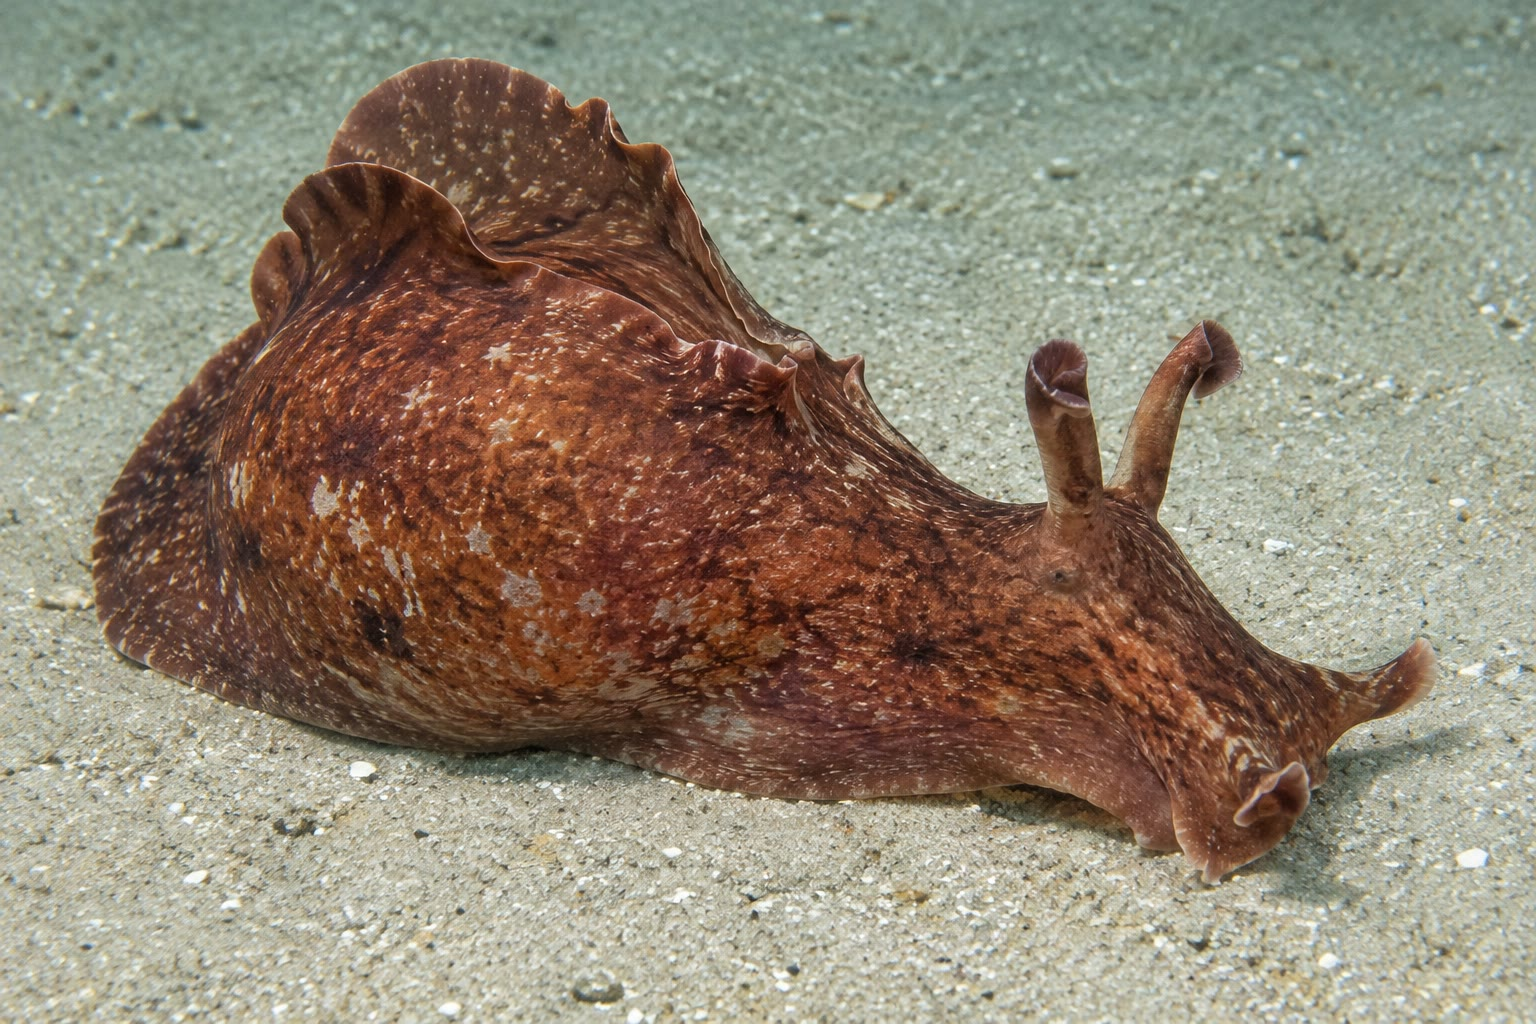
\includegraphics[width=0.46\linewidth]{images/book5/ai/b5-19-aplysia.jpg}\hspace{0.04\linewidth}
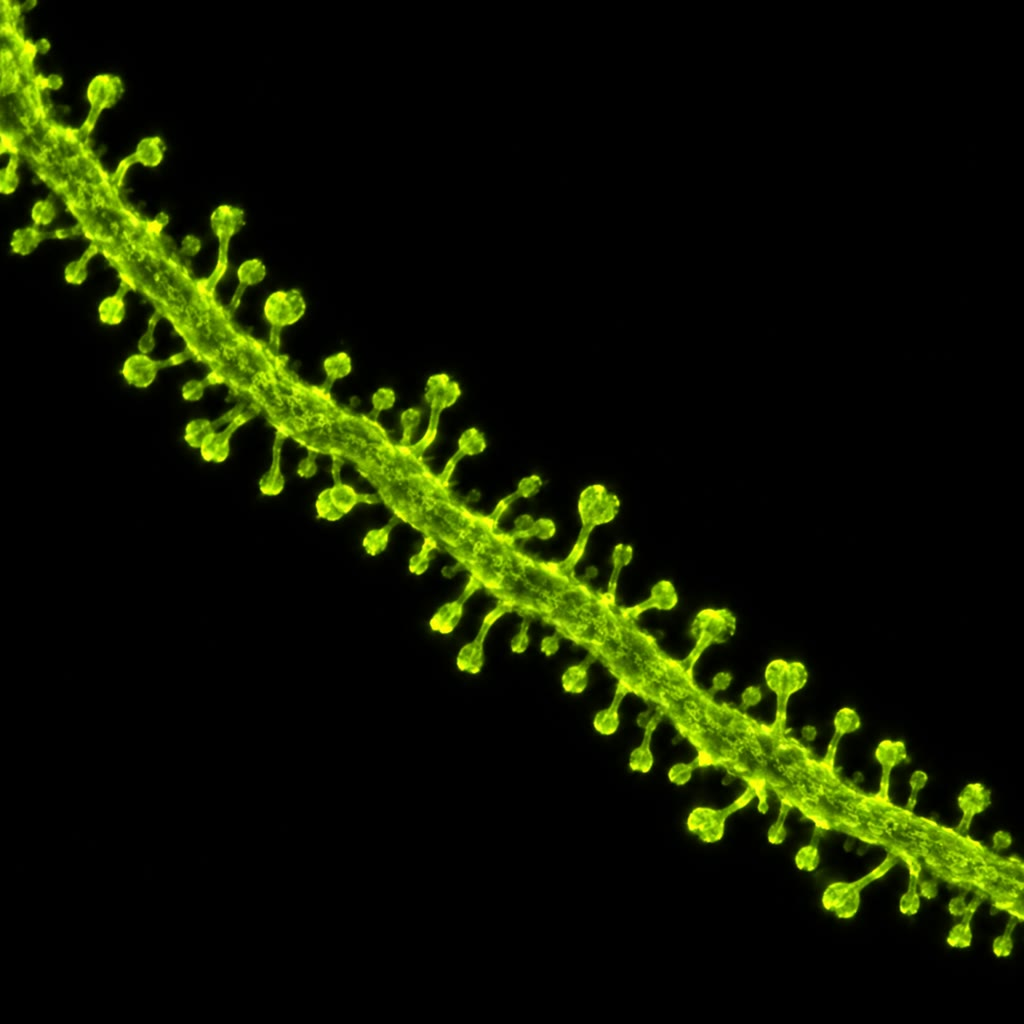
\includegraphics[width=0.36\linewidth]{images/book5/ai/b5-19-dendritic-spines.jpg}

{\small बाएँ: \emph{Aplysia californica}, जिसके थोड़े और बड़े न्यूरॉन
किसी स्मृति की संधि खोजने तथा अभिलिखित करने देते हैं। दाएँ: कंटकों से
जड़ी कोई द्रुमिका, जिनमें से हर एक किसी उत्तेजी संधि का पश्चसंधिक पक्ष
है और हर एक कोई ऐसा कक्ष जिसका कैल्सियम उसकी अपनी नियति तय करता है।}
\end{omfigure}

\section{स्थानों और घटनाओं के परिपथ}

\begin{definition}[हिप्पोकैम्पसी परिपथ]\label{def:b3:learning-memory:hippocampus}
\index{दंतुर कुंडल}\index{CA3}\index{CA1}\index{स्थान कोशिका}\index{जालक कोशिका}\index{प्रतिरूप-पूर्तिकरण}\index{पुनर्चालन}
प्रांतस्थीय निवेश \omterm{def:b3:learning-memory:kinds}{हिप्पोकैम्पस} तक एंटोराइनल प्रांतस्था से होकर पहुँचता
है और तीन चरणों से गुज़रता है: \emph{दंतुर कुंडल}, जिसकी कणिका
कोशिकाएँ अपने निवेशों से अधिक हैं और विरल दगती हैं (जिससे मिलते-जुलते
प्रतिरूप अलग होते हैं); \emph{CA3}, जिसकी पिरामिडी कोशिकाएँ एक-दूसरे से
पुनरावर्ती ढंग से जुड़ी हैं और हर एक दूसरों से हज़ारों संधियाँ पाती है
--- यानी कोई \emph{स्वसाहचर्यी} जाल, जो किसी टुकड़े से कोई संचित
प्रतिरूप पूरा कर सकता है; और \emph{CA1}, जो CA3 के निर्गम की सीधे आते
निवेश से तुलना करता है और परिणाम प्रांतस्था को लौटा देता है। किसी
अखाड़े में घूमते चूहे में \omterm{def:b3:learning-memory:kinds}{हिप्पोकैम्पस} की कोई पिरामिडी कोशिका तभी दगती
है जब वह प्राणी किसी एक जगह हो --- यानी कोई \emph{स्थान कोशिका}
(ओ'कीफ़, 1971) --- और उनमें से कुछ सौ उस अखाड़े का मानचित्र बना देती
हैं; ऊपर एंटोराइनल प्रांतस्था में \emph{जालक कोशिकाएँ} (मोसर, 2005) उस
स्थान को ढँकती किसी षट्कोणीय जालक के शीर्षों पर दगती हैं, यानी कोई
निर्देशांक-तंत्र, जिससे स्थान-क्षेत्र बनाए जाते हैं। नींद और विश्राम के
दौरान उन स्थान कोशिकाओं के क्रम, जो किसी दौड़ के दौरान दगी थीं, तेज़
गति से \emph{पुनर्चालित} किए जाते हैं, और उस पुनर्चालन को रोकने से उस
दौड़ की स्मृति बिगड़ जाती है: \omterm{def:b3:learning-memory:kinds}{हिप्पोकैम्पस} दिन के रास्ते प्रांतस्था को
दुहराकर सुनाता है।
\end{definition}

\begin{omfigure}
\begin{tikzpicture}[every node/.style={font=\scriptsize}, >=stealth]
  % trisynaptic loop
  \node[draw, thick, rounded corners, fill=gray!15, align=center] (ec) at (0,0) {एंटोराइनल प्रांतस्था\\(जालक कोशिकाएँ)};
  \node[draw, thick, rounded corners, fill=omDef!20, align=center] (dg) at (3.2,1.4) {दंतुर कुंडल:\\प्रतिरूप-पृथक्करण};
  \node[draw, thick, rounded corners, fill=omProp!30, align=center] (ca3) at (7.2,1.4) {CA3, पुनरावर्ती:\\प्रतिरूप-पूर्तिकरण};
  \node[draw, thick, rounded corners, fill=omMeth!25, align=center] (ca1) at (7.2,-1.4) {CA1:\\तुलना, निर्गम};
  \draw[->, thick] (ec) -- (dg); \draw[->, thick] (dg) -- (ca3); \draw[->, thick] (ca3) -- (ca1); \draw[->, thick] (ca1) -- (ec) node[pos=0.3, below, sloped, font=\tiny] {प्रांतस्था को वापस};
  \draw[->, thick, dashed] (ec) -- (ca1.north west) node[pos=0.7, above, sloped, font=\tiny] {सीधा पथ};
  \draw[->, thick, omProp!80!black] (ca3.north) .. controls (6.6,2.6) and (7.8,2.6) .. (ca3.north east) node[pos=0.5, above, font=\tiny] {पुनरावर्ती संपार्श्विक};
  % place field map
  \begin{scope}[xshift=10.4cm, yshift=-0.2cm]
    \draw[thick] (0,0) rectangle (3,2.4); \node[below] at (1.5,-0.05) {अखाड़ा, ऊपर से};
    \foreach \p/\c in {(0.7,1.8)/omThm, (2.1,1.9)/omDef, (1.4,0.9)/omMeth, (2.5,0.6)/omProp} { \fill[\c!60] \p circle (0.32); \fill[\c!90] \p circle (0.16); }
    \node[above] at (1.5,2.45) {चार स्थान कोशिकाओं के दगने-क्षेत्र};
  \end{scope}
\end{tikzpicture}

{\small बाएँ: हिप्पोकैम्पसी पाश --- \omterm{def:b3:learning-memory:hippocampus}{दंतुर कुंडल} में पृथक्करण,
पुनरावर्ती \omterm{def:b3:learning-memory:hippocampus}{CA3} में संचयन तथा पूर्तिकरण, \omterm{def:b3:learning-memory:hippocampus}{CA1} में तुलना। दाएँ: हर \omterm{def:b3:learning-memory:hippocampus}{स्थान
कोशिका} किसी अखाड़े के एक ही हिस्से में दगती है; साथ मिलकर वे उस स्थान
का मानचित्र बनाती हैं।}
\end{omfigure}

\begin{proposition}[कोई स्वसाहचर्यी जाल कितना रखता है]\label{prop:b3:learning-memory:capacity}
\index{हॉपफ़ील्ड जाल}\index{स्मृति-क्षमता}
$N$ न्यूरॉनों का कोई जाल, जिसमें हर एक बाकी सबसे हेबीय भारों
$w_{ij} \propto \sum_{\mu}\xi_{i}^{\mu}\xi_{j}^{\mu}$ से जुड़ा हो, जो
संचित द्विआधारी प्रतिरूपों $\xi^{\mu}$ पर जोड़े गए हों, किसी दूषित या
अधूरे संकेत से कोई संचित प्रतिरूप उसी में किसी आकर्षक की तरह जम कर
लौटा देता है (हॉपफ़ील्ड, 1982)। वह ऐसा लगभग $P
\approx 0.14N$ यादृच्छिक प्रतिरूपों तक भरोसे से करता है; उससे आगे
प्रतिरूप एक-दूसरे में दख़ल देते हैं और पुनःप्राप्ति ढह जाती है। किसी
चूहे का \omterm{def:b3:learning-memory:hippocampus}{CA3}, जिसमें कोई $3\times 10^{5}$ पिरामिडी कोशिकाएँ हैं, इस
आकलन पर कोई $4\times 10^{4}$ प्रतिरूप रख सकता है --- यानी उतने ही भिन्न
स्थानों या प्रसंगों की कोटि जितने कोई प्राणी किसी मौसम में मिलता है ---
और उसका विरल दगना (किसी भी प्रतिरूप में कुछ ही प्रतिशत कोशिकाएँ सक्रिय)
उस क्षमता को और बढ़ा देता है। किसी संकेत से प्रतिरूप पूरा कर लेना ही
वह है जिससे कोई गंध या कोई कोना पूरा दृश्य याद दिला देता है; कीमत यह है
कि मिलती-जुलती स्मृतियाँ मिल जाती हैं, जिसका विरोध \omterm{def:b3:learning-memory:hippocampus}{दंतुर कुंडल} का
पृथक्करण करता है।
\end{proposition}
\admitted

\begin{method}[स्मृति और उसके तंत्र की जाँच]\label{met:b3:learning-memory:tests}
\index{मॉरिस जल-भूलभुलैया}\index{भय-अनुबंधन}\index{स्मृतिचिह्न}
(1) कोई स्थानिक कार्य: \omterm{met:b3:learning-memory:tests}{मॉरिस जल-भूलभुलैया} --- कोई चूहा अपारदर्शी पानी
में किसी नियत जगह छिपे मंच तक तैरता है, दिनों भर कमरे के संकेतों से
उसकी जगह सीखता है, और जाँच इससे होती है कि मंच हटाए जाने पर वह सही
चतुर्थांश में कितना समय खोजता है; हिप्पोकैम्पसी क्षतियाँ, NMDA अवरोधक
और LTP का लोप, हर एक उस अधिगम को मिटा देता है। (2) कोई साहचर्यी कार्य:
\omterm{def:b3:learning-memory:kinds}{भय-अनुबंधन} --- किसी पद-झटके से जोड़ा गया कोई स्वर जड़ होना खींचने लगता
है; वह स्मृति अमिग्डला पर टिकी है, और उसका कोई संदर्भ-विशिष्ट रूप
\omterm{def:b3:learning-memory:kinds}{हिप्पोकैम्पस} पर। (3) कोई तंत्र-जाँच: उम्मीदवार को रोकिए (कोई औषध, कोई
ऐसा विलोपन जो एक ही क्षेत्र और समय तक सीमित हो) और दिखाइए कि अधिगम
विफल होता है जबकि प्रत्यक्षण तथा गति नहीं। (4) स्मृतिचिह्न: अधिगम के
दौरान सक्रिय न्यूरॉनों को किसी प्रकाश-संवेदी वाहिका से अंकित कीजिए
(\cref{ch:b3:nervous-systems}) और बाद में उन्हें प्रकाश से फिर सक्रिय
कीजिए --- वह प्राणी किसी सुरक्षित संदर्भ में जड़ हो जाता है, मानो याद
कर रहा हो; और उन्हें चुप कर देने से स्मरण रुक जाता है। स्मृति पहचानी जा
सकने वाली कोशिकाओं और उनकी संधियों में है, और उसे चालू तथा बंद किया जा
सकता है।
\end{method}

\begin{omfigure}
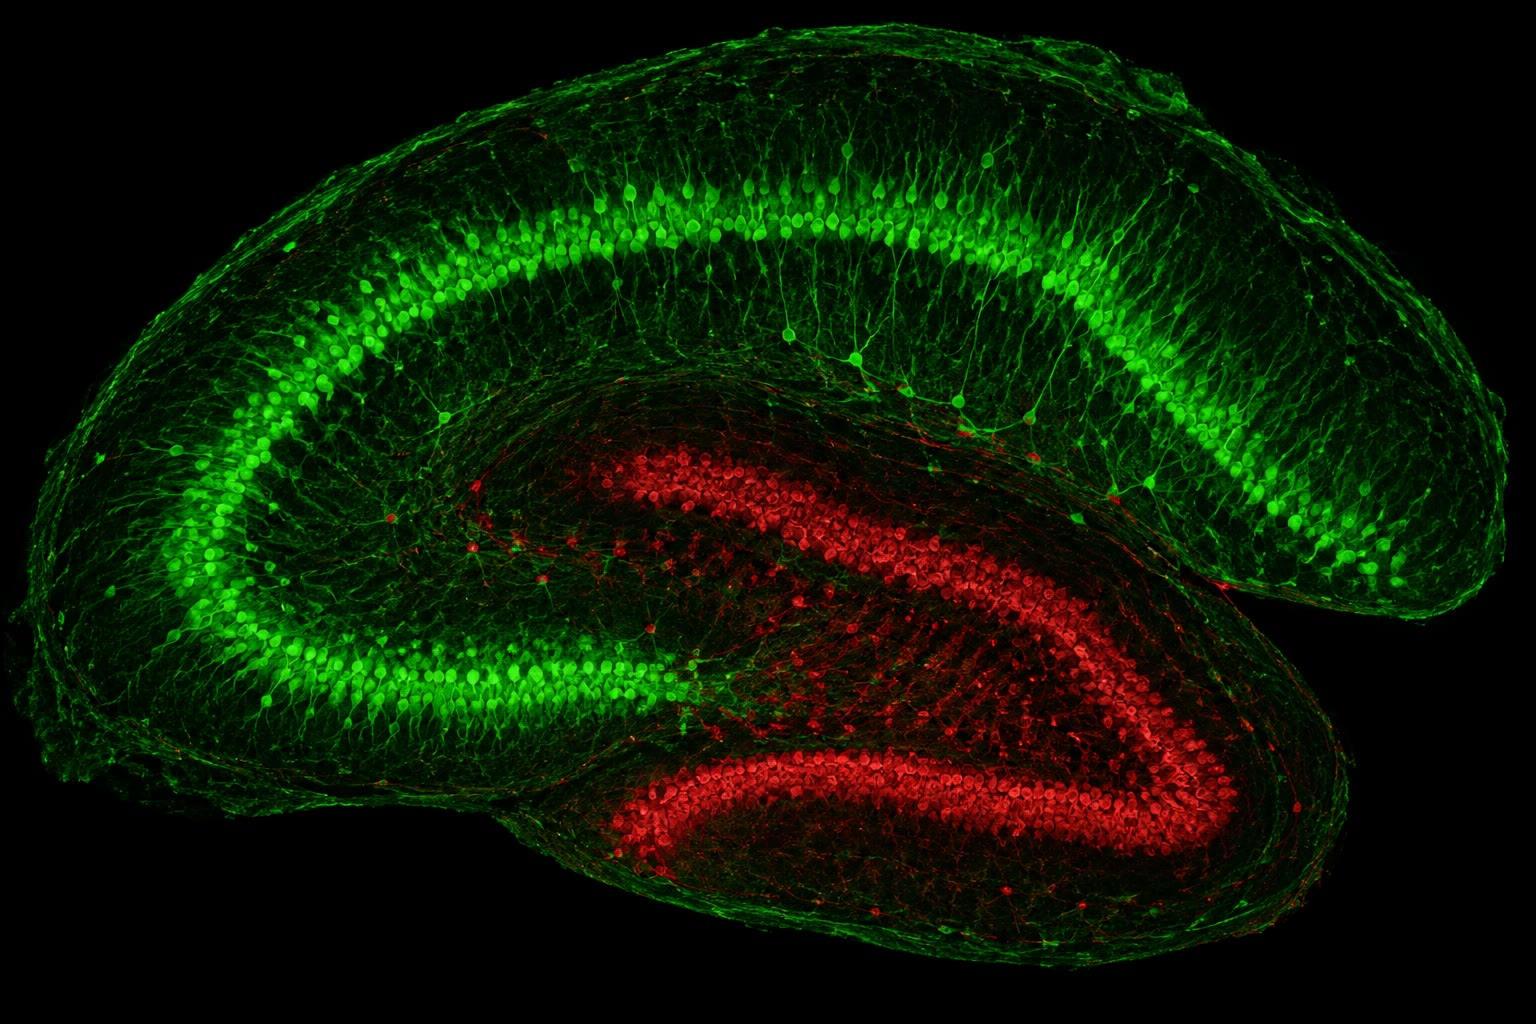
\includegraphics[width=0.56\linewidth]{images/book5/ai/b5-19-hippocampus-section.jpg}

{\small कृंतक \omterm{def:b3:learning-memory:kinds}{हिप्पोकैम्पस} की कोई काट: \omterm{def:b3:learning-memory:hippocampus}{CA3} से \omterm{def:b3:learning-memory:hippocampus}{CA1} तक पिरामिडी
कोशिकाओं की मुड़ी हुई पट्टी (हरी) और उससे गुँथा \omterm{def:b3:learning-memory:hippocampus}{दंतुर कुंडल} (लाल)। उस
प्राणी की हर स्थानिक स्मृति इसी पाश से गुज़रती है।}
\end{omfigure}

\section{पुरस्कार, पूर्वानुमान और जीवन भर की सुघट्यता}

\begin{proposition}[पूर्वानुमान-त्रुटि से अधिगम]\label{prop:b3:learning-memory:rescorla}
\index{रेस्कोर्ला--वैगनर नियम}\index{पूर्वानुमान-त्रुटि}\index{डोपामीन}
मान लीजिए $V$ वह मूल्य है जो कोई प्राणी किसी संकेत से जोड़ता है और
$\lambda$ वह पुरस्कार जो उसके बाद आता है। \omterm{prop:b3:learning-memory:rescorla}{रेस्कोर्ला--वैगनर नियम} (1972)
कहता है कि हर आज़माइश पर वह मूल्य \emph{पूर्वानुमान-त्रुटि} के किसी
अंश $\alpha$ से बदलता है:
\[
\Delta V = \alpha\,(\lambda - V), \qquad
V_{n} = \lambda\bigl(1 - (1-\alpha)^{n}\bigr) ,
\]
इसलिए अधिगम पहले तेज़ होता है और पूर्वानुमान सुधरने पर धीमा पड़ता है,
पुरस्कार के पूरी तरह पूर्वानुमानित हो जाने पर रुक जाता है, और पुरस्कार
रोक दिए जाने पर पलट जाता है (विलोपन)। जब दो संकेत साथ प्रस्तुत हों तब
वे एक ही पूर्वानुमान साझा करते हैं, इसलिए जो संकेत पहले से बने किसी
पूर्वानुमान में कुछ न जोड़े वह सीखा ही नहीं जाता (\emph{अवरोधन})।
शुल्ट्स (1997) ने बंदरों के मध्यमस्तिष्क के डोपामीन न्यूरॉन अभिलिखित
किए और पाया कि वे किसी अप्रत्याशित पुरस्कार पर दगते हैं, किसी पूरी तरह
पूर्वानुमानित पर चुप हो जाते हैं, और जब कोई पूर्वानुमानित पुरस्कार न आए
तब आधार-रेखा से नीचे गिर जाते हैं: वे $\lambda - V$, यानी स्वयं वह
पूर्वानुमान-त्रुटि, धारीदार पिंड तथा प्रांतस्था तक प्रसारित करते हैं,
जहाँ डोपामीन उन संधियों पर सुघट्यता का द्वार खोलता है जो हाल में सक्रिय
थीं। यह सीखना कि क्या पुरस्कार का पूर्वानुमान करता है, कोई हेबीय
सुघट्यता है जिसमें कोई तीसरा गुणक यह बताता है कि परिणाम प्रत्याशा से
बेहतर था या बुरा --- और दुरुपयोग की औषधें, डोपामीन सीधे चलाकर, किसी
स्थायी ``प्रत्याशा से बेहतर'' की जालसाज़ी कर देती हैं।
\end{proposition}
\begin{proof}
पुनरावर्तन $V_{n+1} = V_{n} + \alpha(\lambda - V_{n})$ देता है
$\lambda - V_{n+1} = (1-\alpha)(\lambda - V_{n})$, इसलिए वह त्रुटि
गुणोत्तर ढंग से सिकुड़ती है, $\lambda - V_{n} = (1-\alpha)^{n}\lambda$,
जहाँ $V_{0} =
0$, जिससे वह सूत्र निकलता है। साथ प्रस्तुत किए गए दो संकेतों $A$ और $B$ के लिए
पूर्वानुमान $V_{A} + V_{B}$ है; यदि $A$ को पहले
$V_{A} = \lambda$ तक प्रशिक्षित किया गया हो, तो संयुक्त आज़माइशों पर
त्रुटि शून्य है और $B$ कुछ भी नहीं पाता।
\end{proof}

\begin{omfigure}
\begin{tikzpicture}
\begin{axis}[
  width=6.6cm, height=5.0cm,
  axis x line=bottom, axis y line=left,
  xmin=0, xmax=25, ymin=0, ymax=1.1,
  xlabel={आज़माइश $n$}, ylabel={$V_{n}/\lambda$},
  xlabel style={font=\small, at={(axis description cs:0.5,-0.14)}, anchor=north}, ylabel style={font=\small},
  tick label style={font=\scriptsize}, xtick={0,5,10,15,20,25}, ytick={0,0.5,1},
  clip=false,
]
\addplot[very thick, omDef, domain=0:12, samples=13] {1-0.8^x};
\addplot[very thick, omDef, domain=12:25, samples=14] {(1-0.8^12)*0.8^(x-12)};
\draw[dashed, gray] (axis cs:12,0) -- (axis cs:12,1.05);
\node[font=\scriptsize, anchor=north west, align=left] at (axis cs:0.5,0.98) {पुरस्कार दिया गया:\\अर्जन};
\node[font=\scriptsize, anchor=north west, align=left] at (axis cs:14,0.98) {पुरस्कार रोका गया:\\विलोपन};
\end{axis}
\begin{axis}[
  at={(7.6cm,0)}, anchor=south west,
  width=6.6cm, height=5.0cm,
  ybar, bar width=14pt,
  axis x line=bottom, axis y line=left,
  ymin=-1.2, ymax=1.5,
  symbolic x coords={unexpected reward, predicted reward, reward omitted},
  xtick=data, ytick={-1,0,1}, yticklabels={गिरावट,आधार-रेखा,झोंका},
  xticklabels={{अप्रत्याशित पुरस्कार},{पूर्वानुमानित पुरस्कार},{पुरस्कार छोड़ा गया}},
  ylabel={डोपामीन का दगना},
  x tick label style={font=\scriptsize, align=center, text width=1.9cm}, ylabel style={font=\small}, tick label style={font=\scriptsize},
  clip=false,
]
\addplot[fill=omThm!50, draw=omThm] coordinates {(unexpected reward,1.2) (predicted reward,0.05) (reward omitted,-1.0)};
\end{axis}
\end{tikzpicture}

{\small बाएँ: $\alpha = 0.2$ के साथ रेस्कोर्ला--वैगनर अधिगम-वक्र ---
पुरस्कार के मूल्य तक गुणोत्तर पहुँच, फिर पुरस्कार रुकने पर विलोपन।
दाएँ: डोपामीन न्यूरॉन पूर्वानुमान-त्रुटि बताते हैं --- किसी अचरज पर
कोई झोंका, किसी पूर्वानुमानित पुरस्कार पर कुछ नहीं, और कोई
पूर्वानुमानित पुरस्कार चूकने पर कोई गिरावट।}
\end{omfigure}

\begin{definition}[क्रांतिक काल और सुघट्यता के रोग]\label{def:b3:learning-memory:critical}
\index{क्रांतिक काल}\index{नेत्र-प्रभुत्व}\index{व्यसन}\index{अल्ज़ाइमर रोग}
सुघट्यता परिवर्धन की खिड़कियों में सबसे अधिक होती है। ह्यूबेल और
वीज़ेल (1960 का दशक) ने किसी बिल्ली के बच्चे की एक आँख जन्म के बाद कुछ
हफ़्तों तक ढँक दी: दृष्टि प्रांतस्था, जो सामान्यतः बारी-बारी के स्तंभों
में दोनों आँखों से चलती है, लगभग पूरी तरह खुली आँख से चलने लगी, और वह
वंचित आँख जीवन भर प्रकार्यतः अंधी रह गई --- जबकि किसी वयस्क बिल्ली में
वही वंचन कुछ नहीं बदलता। ऐसे \emph{क्रांतिक काल}, दृष्टि के लिए, भाषा
के लिए, पक्षियों के गीतों के लिए, तब बंद होते हैं जब निरोधी परिपथ
परिपक्व होते हैं और बाह्यकोशिकीय आधात्री कड़ी पड़ जाती है, और उन्हें
औषधों तथा प्रशिक्षण से थोड़ा फिर खोला जा सकता है। सुघट्यता की व्याधियाँ
मात्रा और लक्ष्य की हैं: \emph{व्यसन} किसी जाली पूर्वानुमान-त्रुटि से
चलता अधिगम है, जो ऐसी आदतें बनाता है जो उस सुख से भी आगे टिकती हैं;
अभिघातोत्तर तनाव कोई ऐसी भय-स्मृति है जिसे तनाव-हॉर्मोनों ने कुछ अधिक
ही सुदृढ़ कर दिया हो; और \emph{अल्ज़ाइमर रोग} वहीं शुरू होता है जहाँ
\omterm{def:b3:learning-memory:kinds}{घोषणात्मक स्मृति} शुरू होती है, यानी एंटोराइनल प्रांतस्था और
\omterm{def:b3:learning-memory:kinds}{हिप्पोकैम्पस} में, तंत्रिका-संधियों के लोप से --- जो किसी भी पट्टिका-गणना
से बेहतर उस मनोभ्रंश का पीछा करता है --- और यह न्यूरॉनों के लोप से पहले।
\end{definition}

\begin{remark}[स्मृति किस चीज़ की बनी है]\label{rem:b3:learning-memory:what}
कोई स्मृति कोई अभिलेखन नहीं, बल्कि तंत्रिका-संधियों के बलों तथा
संख्याओं का कोई बदलाव है, जो उन कोशिकाओं भर में बँटा है जो उसके बनते
समय सक्रिय थीं, जो किसी ऐसे नियम से बिछाया गया है जो साथ दगते को
मज़बूत करता है, जिसका द्वार कोई ऐसा संकेत खोलता है जो बताता है कि
परिणाम मायने रखता था या नहीं, और जिसका अभ्यास नींद में तब तक होता है जब
तक प्रांतस्था उसे अपने बूते न थाम ले। वह नियम हेब का है, वह द्वार \omterm{prop:b3:learning-memory:nmda}{NMDA
ग्राही}, वह संकेत डोपामीन, वह अभ्यास \omterm{def:b3:learning-memory:hippocampus}{पुनर्चालन}, और वह गणित बताता है कि
ऐसा कोई तंत्र कितना रख सकता है और वह मिलते-जुलते को क्यों गड्डमड्ड कर
देता है। जिस भी प्रयोग ने कोई स्मृति चालू या बंद की है --- किसी
अवरोधक, किसी जीन, किसी प्रकाश से --- उसने उसे उन्हीं संधियों में, उन्हीं
कोशिकाओं में पाया है। H.M. 2008 में मरा; उसका मस्तिष्क, काटकर और
प्रतिबिंबित करके, वही क्षति दिखा गया जिसने उस क्षेत्र को पढ़ाया था, और
इससे अधिक कुछ नहीं।
\end{remark}

\section{अभ्यास}

\begin{exercise}[$\star$]\label{exo:b3:learning-memory:1}
H.M. के निष्पादन से घोषणात्मक और अघोषणात्मक स्मृति में भेद कीजिए, और
अघोषणात्मक स्मृति के चार प्रकारों में से हर एक के लिए मस्तिष्क का एक-एक
क्षेत्र बताइए।
\end{exercise}

\begin{exercise}[$\star$]\label{exo:b3:learning-memory:2}
हेब का अभिगृहीत बताइए और LTP के वे तीन गुण जो उससे निकलते हैं।
\end{exercise}

\begin{exercise}[$\star$]\label{exo:b3:learning-memory:3}
समझाइए कि \omterm{prop:b3:learning-memory:nmda}{NMDA ग्राही} कोई संपात-संसूचक क्यों है, और उसका अवरोधक AP5
टेटेनस से पहले तथा उसके बाद लगाने पर LTP का क्या होता है।
\end{exercise}

\begin{exercise}[$\star$]\label{exo:b3:learning-memory:4}
\emph{Aplysia} में आणविक स्तर पर अल्पकालिक को दीर्घकालिक \omterm{def:b3:learning-memory:kinds}{संवेदीकरण} से
क्या अलग करता है, और कौन-सा प्रयोग यह दिखाता है?
\end{exercise}

\begin{exercise}[$\star\star$]\label{exo:b3:learning-memory:5}
$\alpha = 0.3$ के साथ, $V$ को $\lambda$ के \qty{90}{\%} तक पहुँचने में
कितनी आज़माइशें लगती हैं? यदि फिर पुरस्कार रोक दिया जाए, तो $V$ को
\qty{10}{\%} से नीचे गिरने में कितनी? इस प्रतिरूप में अर्जन और विलोपन
सममित क्यों हैं, और क्या वे प्राणियों में भी हैं?
\end{exercise}

\begin{exercise}[$\star\star$]\label{exo:b3:learning-memory:6}
दो निवेशों का $C = \begin{pmatrix}1 & 0.5\\ 0.5 & 1\end{pmatrix}$ है।
अभिलक्षणिक सदिश और अभिलक्षणिक मान खोजिए, और बताइए कि \omterm{def:b3:learning-memory:ltp}{हेब का नियम} भारों
को किस दिशा की ओर मोड़ता है और वह न्यूरॉन फिर क्या पकड़ता है। \omterm{thm:b3:learning-memory:hebb}{ओया का नियम}
$\mathbf{w} = (1,0)$ से एक पग के लिए लगाइए, निवेश $\mathbf{x}
= (1,1)$ और $\eta = 0.1$ के साथ।
\end{exercise}

\begin{exercise}[$\star\star$]\label{exo:b3:learning-memory:7}
किसी कंटक का आयतन \qty{0.1}{fL} है। $500$ कैल्सियम आयनों का प्रवेश
उसकी मुक्त सांद्रता कितनी बढ़ा देता है ($\unit{\micro mol/L}$ में),
यदि \qty{95}{\%} तुरंत बफ़रों से बँध जाएँ? विश्रामी
\qty{0.1}{\micro mol/L} से और CaMKII के सक्रियक कैल्मॉड्युलिन के
$K_{d}$ से, जो लगभग \qty{1}{\micro mol/L} है, तुलना कीजिए।
\end{exercise}

\begin{exercise}[$\star\star$]\label{exo:b3:learning-memory:8}
\omterm{prop:b3:learning-memory:rescorla}{रेस्कोर्ला--वैगनर नियम} से अवरोधन समझाइए और हर चरण के लिए उससे मेल खाता
डोपामीन-अभिलेख दीजिए।
\end{exercise}

\begin{exercise}[$\star\star$]\label{exo:b3:learning-memory:9}
इनके परिणामों का पूर्वानुमान कीजिए: (क) \omterm{def:b3:learning-memory:hippocampus}{CA1} तक सीमित \omterm{prop:b3:learning-memory:nmda}{NMDA ग्राही} का
विलोपन, (ख) प्रशिक्षण के दौरान दिया गया कोई प्रोटीन-संश्लेषण निरोधक,
(ग) वही निरोधक एक दिन बाद दिया गया, (घ) किसी \omterm{def:b3:learning-memory:kinds}{भय-अनुबंधन} के दौरान सक्रिय
रही दंतुर-कुंडल कोशिकाओं का किसी नए संदर्भ में प्रकाश-आनुवंशिक
पुनःसक्रियण।
\end{exercise}

\begin{exercise}[$\star\star\star$]\label{exo:b3:learning-memory:10}
दिखाइए कि अकेले हेब के नियम के अंतर्गत $\mathbf{w}$ की लंबाई बिना किसी
सीमा के बढ़ती है, और ओया के नियम में किसी भी स्थिर बिंदु पर
$|\mathbf{w}| = 1$ होता है। असीम वृद्धि कोई जैविक समस्या क्यों है, और
कौन-से तंत्र (संधि-मापक्रमण, LTD, नींद) उस अभिसामान्यक पद से मेल खा
सकते हैं?
\end{exercise}

\begin{exercise}[$\star\star\star$]\label{exo:b3:learning-memory:11}
किसी चूहे के \omterm{def:b3:learning-memory:hippocampus}{CA3} में $3\times 10^{5}$ कोशिकाएँ हैं; किसी मनुष्य के में
लगभग $2\times 10^{6}$। हर एक की हॉपफ़ील्ड क्षमता आँकिए। यह आकलन इस बात
का खराब माप क्यों है कि कोई व्यक्ति कितनी स्मृतियाँ रखता है, और
\omterm{def:b3:learning-memory:kinds}{सुदृढ़ीकरण} में \omterm{def:b3:learning-memory:kinds}{हिप्पोकैम्पस} की भूमिका इस चित्र में क्या जोड़ती है?
\end{exercise}

\begin{exercise}[$\star\star\star$]\label{exo:b3:learning-memory:12}
जिन बिल्ली के बच्चों की एक आँख की दृष्टि हफ़्तों तक वंचित रहे वे उस
आँख का प्रांतस्थीय इलाक़ा खो देते हैं; वयस्क नहीं। हेबीय स्पर्धा से
समझाइए कि खुली आँख क्यों जीतती है, दोनों आँखों का वंचन एक के वंचन से
कम असर क्यों करता है, और वह \omterm{def:b3:learning-memory:critical}{क्रांतिक काल} किससे बंद होता है।
\end{exercise}

\section{समस्या: एक संधि जो याद रखती है}

\begin{problem}[{सप्तांत समस्या --- किसी कंटक के कैल्सियम से लेकर किसी
भूलभुलैया के चूहे तक पीछा की गई कोई स्मृति: प्रेरण का कैल्सियम-अंकगणित,
कोई हेबीय न्यूरॉन जो अपने निवेशों की साझा बात पर अभिसरित होता है,
पूर्वानुमान-त्रुटि से समयबद्ध कोई अधिगम-वक्र, और किसी हिप्पोकैम्पस की
क्षमता, जिसका अंत उस कैल्सियम सांद्रता पर होता है जो LTP प्रेरित करती
है, उन आज़माइशों पर जो किसी चूहे को चाहिए, और उन प्रतिरूपों पर जो उसका
CA3 रख सकता है}]
\label{pb:b3:learning-memory:1}
आँकड़े: \qty{0.08}{fL} आयतन का कोई कंटक; हर NMDA वाहिका \qty{50}{ms}
के हर खुलने पर $10^{3}$ Ca$^{2+}$ ढोती है; किसी संधि के $10$ \omterm{prop:b3:learning-memory:nmda}{NMDA
ग्राही} हैं; भीतर आते कैल्सियम का \qty{98}{\%} बफ़रित होता है; विश्रामी
मुक्त कैल्सियम \qty{0.1}{\micro mol/L}; CaMKII
\qty{2}{\micro mol/L} मुक्त कैल्सियम से ऊपर सक्रिय होती है, और
कैल्सिन्यूरिन $0.3$ तथा
\qty{1}{\micro mol/L} के बीच। हेब: दो निवेश, जिनका $C = \begin{pmatrix}1 &
0.6\\ 0.6 & 1\end{pmatrix}$, $\eta = 0.1$। रेस्कोर्ला--वैगनर: $\alpha =
0.15$। क्षमता: चूहे का \omterm{def:b3:learning-memory:hippocampus}{CA3} $3\times 10^{5}$ कोशिकाएँ, $P = 0.14N$; कोई
चूहा दिन में $20$ नई जगहें घूमता है।

\medskip
\noindent\textbf{भाग I --- कैल्सियम।}
\begin{enumerate}
  \item दसों \omterm{prop:b3:learning-memory:nmda}{NMDA ग्राही} एक-एक बार खुलते हैं। कितने कैल्सियम आयन भीतर
        आते हैं, कितने मुक्त रहते हैं, और उस कंटक में वह कितनी
        सांद्रता-वृद्धि हुई?
  \item क्या CaMKII सक्रिय होती है? और यदि केवल दो ग्राही खुलें
        (ग्लूटामेट छूटा पर वह कंटक मुश्किल से विध्रुवित हुआ)?
  \item दो ग्राही खुलने पर कौन-सी एंज़ाइम अपनी परास में है, और उस संधि
        का क्या होता है? समझाइए कि कोई एक आयन LTP और LTD, दोनों कैसे
        पैदा कर सकता है।
  \item कैल्सियम \qty{20}{ms} के किसी काल-अचर से बाहर पंप किया जाता
        है। निवेशों को अपना कैल्सियम जोड़ने के लिए दसियों मिलीसेकंडों
        के भीतर क्यों पहुँचना पड़ता है, और इससे आवेग-काल की खिड़की कैसे
        तय होती है?
  \item कोई कंटक द्रुमिका पर अपने पड़ोसी से \qty{0.5}{\micro m} दूर
        है। समझाइए कि बफ़रण और उस कंटक की सँकरी गर्दन वह कैल्सियम-संकेत
        एक ही कंटक में क्यों रखते हैं, और यह निवेश-विशिष्टता के लिए
        क्यों मायने रखता है।
  \item मैग्नीशियम अवरोध लगभग \qty{-30}{mV} पर हटता है। कोई अकेली AMPA
        संधि उस कंटक को \qty{-70}{mV} से \qty{5}{mV} विध्रुवित करती
        है। \omterm{prop:b3:learning-memory:nmda}{NMDA ग्राही} खुलवाने के लिए कितने समकालिक निवेश (या और क्या)
        चाहिए? इससे \omterm{def:b3:structural-biology:allostery}{सहकारिता} के बारे में क्या निकलता है?
\end{enumerate}

\medskip
\noindent\textbf{भाग II --- कोई हेबीय न्यूरॉन।}
\begin{enumerate}[resume]
  \item $C$ के अभिलक्षणिक मान और अभिलक्षणिक सदिश खोजिए।
  \item $\mathbf{w} = (1, 0)$ से शुरू करके, औसत हेब नियम
        $\mathbf{w} \leftarrow \mathbf{w} + \eta C\mathbf{w}$ तीन पगों
        के लिए लगाइए। हर पग के बाद $\mathbf{w}$ का $(1,1)$ दिशा से
        कोण क्या है?
  \item अनेक पगों के बाद अनुपात $w_{2}/w_{1}$ क्या है, और
        $|\mathbf{w}|$ का क्या होता है?
  \item ओया का औसत नियम $\mathbf{w} \leftarrow \mathbf{w} +
        \eta\,(C\mathbf{w} - (\mathbf{w}^{\mathsf{T}}C\mathbf{w})
        \mathbf{w})$ $(0.8, 0.8)$ से एक पग के लिए लगाइए। वह किस ओर
        बढ़ता है?
  \item वह न्यूरॉन अब दोनों निवेशों पर साथ अनुक्रिया देता है। यदि केवल
        निवेश 2 दगे (जो बिरला है), तो संयुक्त स्थिति के सापेक्ष $y$
        क्या है, $\mathbf{w} = (0.71, 0.71)$ के साथ?
  \item एक वाक्य में समझाइए कि LTP की साहचर्यिता (किसी प्रबल के साथ
        जोड़ा गया कोई दुर्बल निवेश मज़बूत होता है) यही प्रमेय काम करते
        हुए कैसे है।
\end{enumerate}

\medskip
\noindent\textbf{भाग III --- अधिगम-वक्र।}
\begin{enumerate}[resume]
  \item $\alpha = 0.15$ के साथ, $V_{n}/\lambda$ निकालिए, $5$, $10$ और
        $20$ आज़माइशों के बाद।
  \item $\lambda$ के \qty{95}{\%} तक पहुँचने में कितनी आज़माइशें?
  \item कोई चूहा लगभग इतनी ही आज़माइशों में कोई भूलभुलैया सीख लेता है।
        यदि पुरस्कार दुगुना कर दिया जाए, तो क्या वह प्रतिरूप
        आज़माइशों में तेज़ अधिगम का पूर्वानुमान करता है? क्या बदलता है?
  \item संकेत A को अनंतस्पर्शी तक प्रशिक्षित किया जाता है, फिर A और B
        उसी पुरस्कार के साथ $20$ आज़माइशों तक साथ प्रस्तुत किए जाते
        हैं। $V_{B}$ क्या है? संयुक्त आज़माइशों पर डोपामीन न्यूरॉन
        क्या करते हैं?
  \item अब पुरस्कार अकेले B के बाद आता है। पहली आज़माइश की
        पूर्वानुमान-त्रुटि तथा डोपामीन-अनुक्रिया, और $V_{B}$ की चाल का
        वर्णन कीजिए।
  \item कोई औषध परिणाम चाहे जो हो, डोपामीन बढ़ा देती है। उस नियम से
        समझाइए कि उस औषध से पहले की क्रियाएँ, उनके नतीजे जो भी हों,
        क्यों पुरस्कृत जैसी सीखी जाती हैं।
\end{enumerate}

\medskip
\noindent\textbf{भाग IV --- \omterm{def:b3:learning-memory:kinds}{हिप्पोकैम्पस}।}
\begin{enumerate}[resume]
  \item चूहे के \omterm{def:b3:learning-memory:hippocampus}{CA3} की हॉपफ़ील्ड क्षमता।
  \item दिन में $20$ नई जगहों पर, वह क्षमता भरने में कितना समय लगेगा?
        उस प्राणी के सीखते रहने के लिए क्या होना चाहिए?
  \item \omterm{def:b3:learning-memory:kinds}{सुदृढ़ीकरण} स्मृतियाँ हफ़्तों में प्रांतस्था तक पहुँचा देता है।
        समझाइए कि कोई धीमा अंतरण पुरानी प्रांतस्थीय स्मृतियों की रक्षा
        क्यों करता है (विनाशकारी दख़ल) और \omterm{def:b3:learning-memory:kinds}{हिप्पोकैम्पस} कोई अस्थायी
        भंडार क्यों है।
  \item यदि किसी भी प्रतिरूप में \omterm{def:b3:learning-memory:hippocampus}{CA3} की \qty{3}{\%} कोशिकाएँ सक्रिय
        हों, तो कोई एक स्थान कितनी कोशिकाएँ कूटबद्ध करती हैं, और यदि
        प्रतिरूपों को अपनी आधी से कम कोशिकाएँ साझा करनी पड़ें तो कितने
        प्रतिरूप अलग पहचाने जा सकते? (गुणात्मक रूप से तर्क दीजिए कि
        विरल कूटलेखन क्षमता क्यों बढ़ाता है।)
  \item नींद में \omterm{def:b3:learning-memory:hippocampus}{पुनर्चालन} किसी \qty{10}{s} की दौड़ को \qty{0.5}{s} में
        निचोड़ देता है। यदि आवेग-काल की खिड़की \qty{20}{ms} हो, तो उस
        दौड़ में \omterm{def:b3:learning-memory:hippocampus}{स्थान कोशिकाओं} के दगने की कौन-सी दूरी \omterm{def:b3:learning-memory:hippocampus}{पुनर्चालन} में
        हेबीय बन जाती है? इस निचोड़ का यही मतलब क्यों हो सकता है?
  \item भूलभुलैया की वह स्मृति प्रशिक्षण के महीने भर बाद की गई
        हिप्पोकैम्पसी क्षति झेल जाती है पर दिन भर बाद की नहीं। H.M. के
        लोप के ढर्रे से इसकी व्याख्या कीजिए।
  \item सारांश दीजिए: दस NMDA खुलनों के बाद मुक्त कैल्सियम की सांद्रता
        (प्रश्न~1), \qty{95}{\%} अधिगम तक की आज़माइशें (प्रश्न~14), और
        चूहे के \omterm{def:b3:learning-memory:hippocampus}{CA3} की क्षमता (प्रश्न~19)।
\end{enumerate}
\end{problem}
